
\begin{frame}
  Finding genes that are differentially expressed (\mywarn{shift of the mean}) under
  different conditions. 
  \begin{columns}
    \begin{column}{0.6\textwidth}
      \begin{figure}
        \centering
        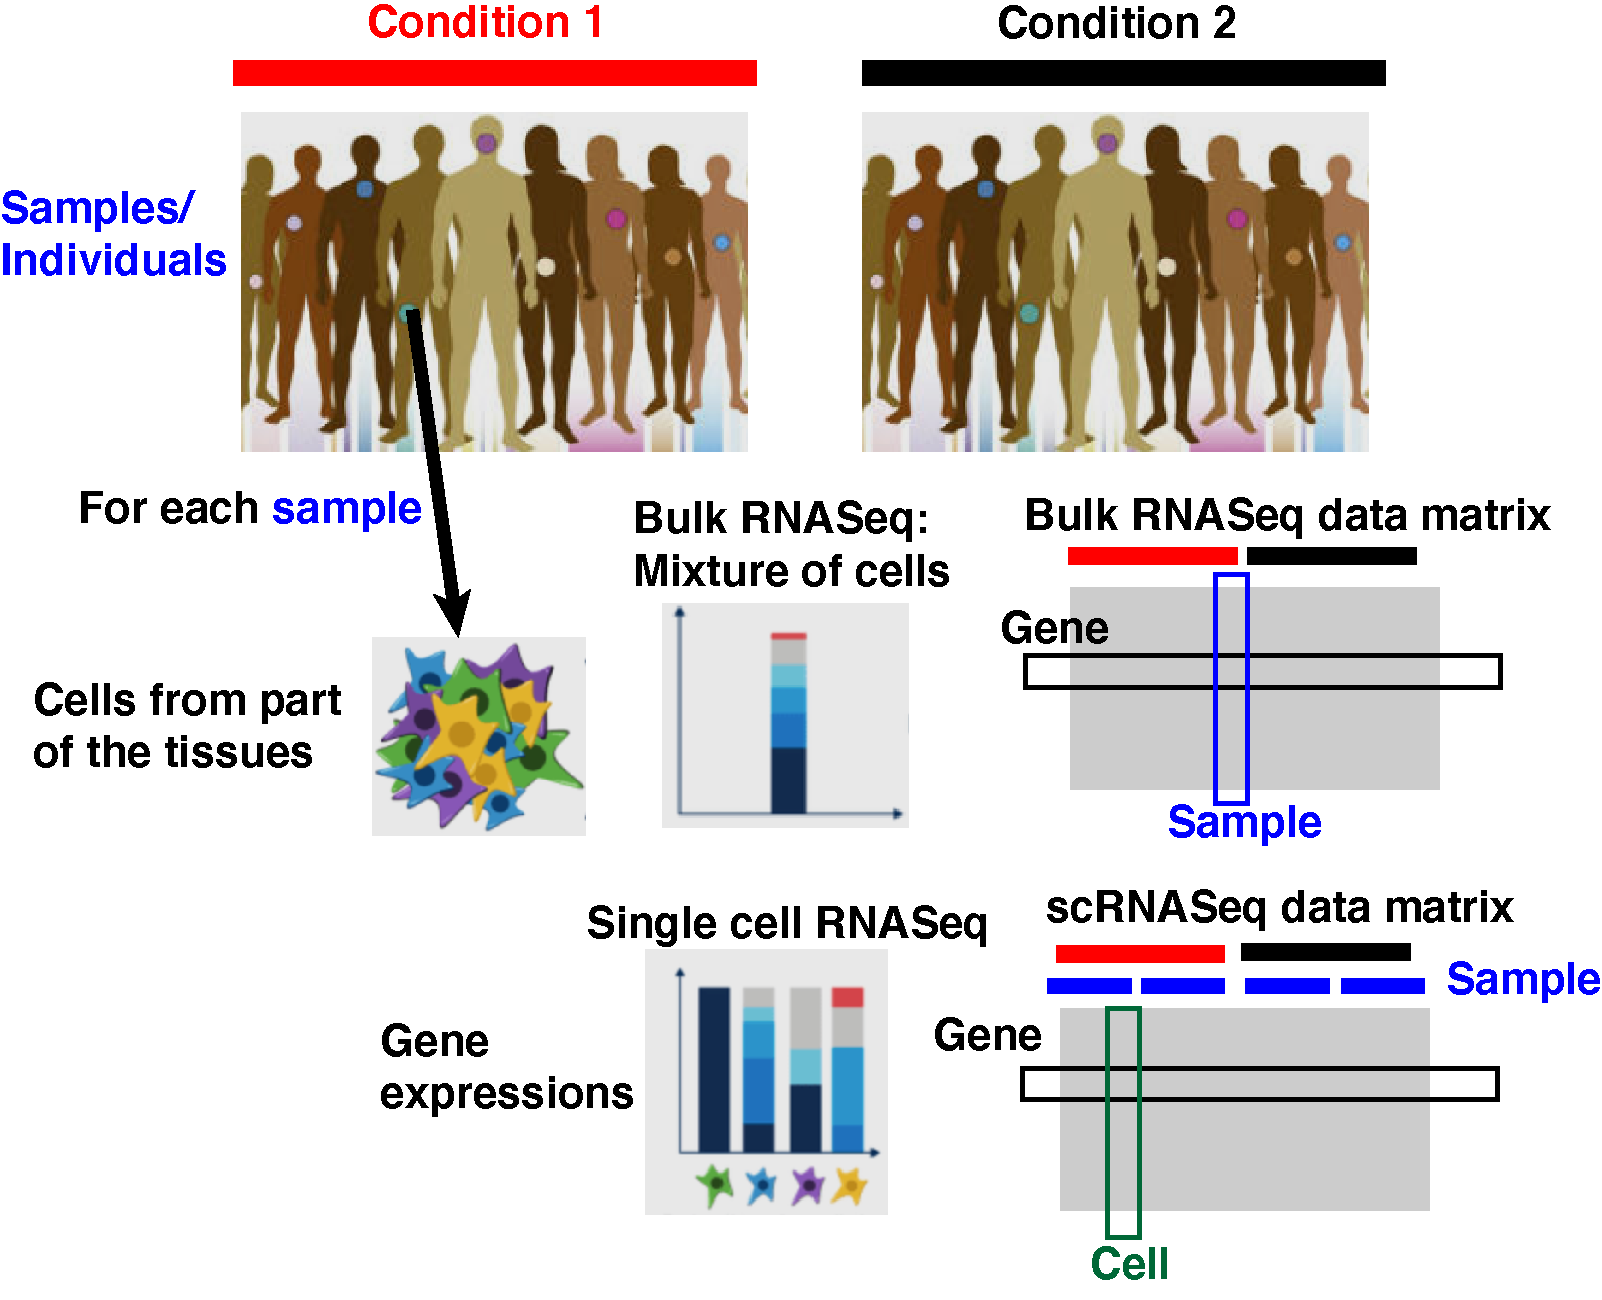
\includegraphics[width = \textwidth]{background_explain}
      \end{figure}
    \end{column}
    \begin{column}{0.45\textwidth}
      \begin{itemize}
      \item Bulk RNASeq: \\the gene \(i\) in the sample \(j\)
        \({\scriptstyle \log_2CPM(X_{ij}) = \log_2(1 + X_{ij} \cdot S_{j}) }\) \\
        \({\scriptstyle S_j =\frac{1}{\sum_{i} X_{ij}} \cdot 10^6}\)
    \item UMI-based scRNAseq
      \begin{itemize}
      \item Data: 70\% zeros
      \item Limited samples
      \item Technical variations:\\
        1. Batch effect\\
        2. scRNA sequencing
      \item Biological variations:\\
        1. Genetic background \\
        2. Cell heterogeneity
         \end{itemize}
      \end{itemize}
    \end{column}
  \end{columns}
\end{frame}

\begin{frame}
  \begin{figure}
    \centering
    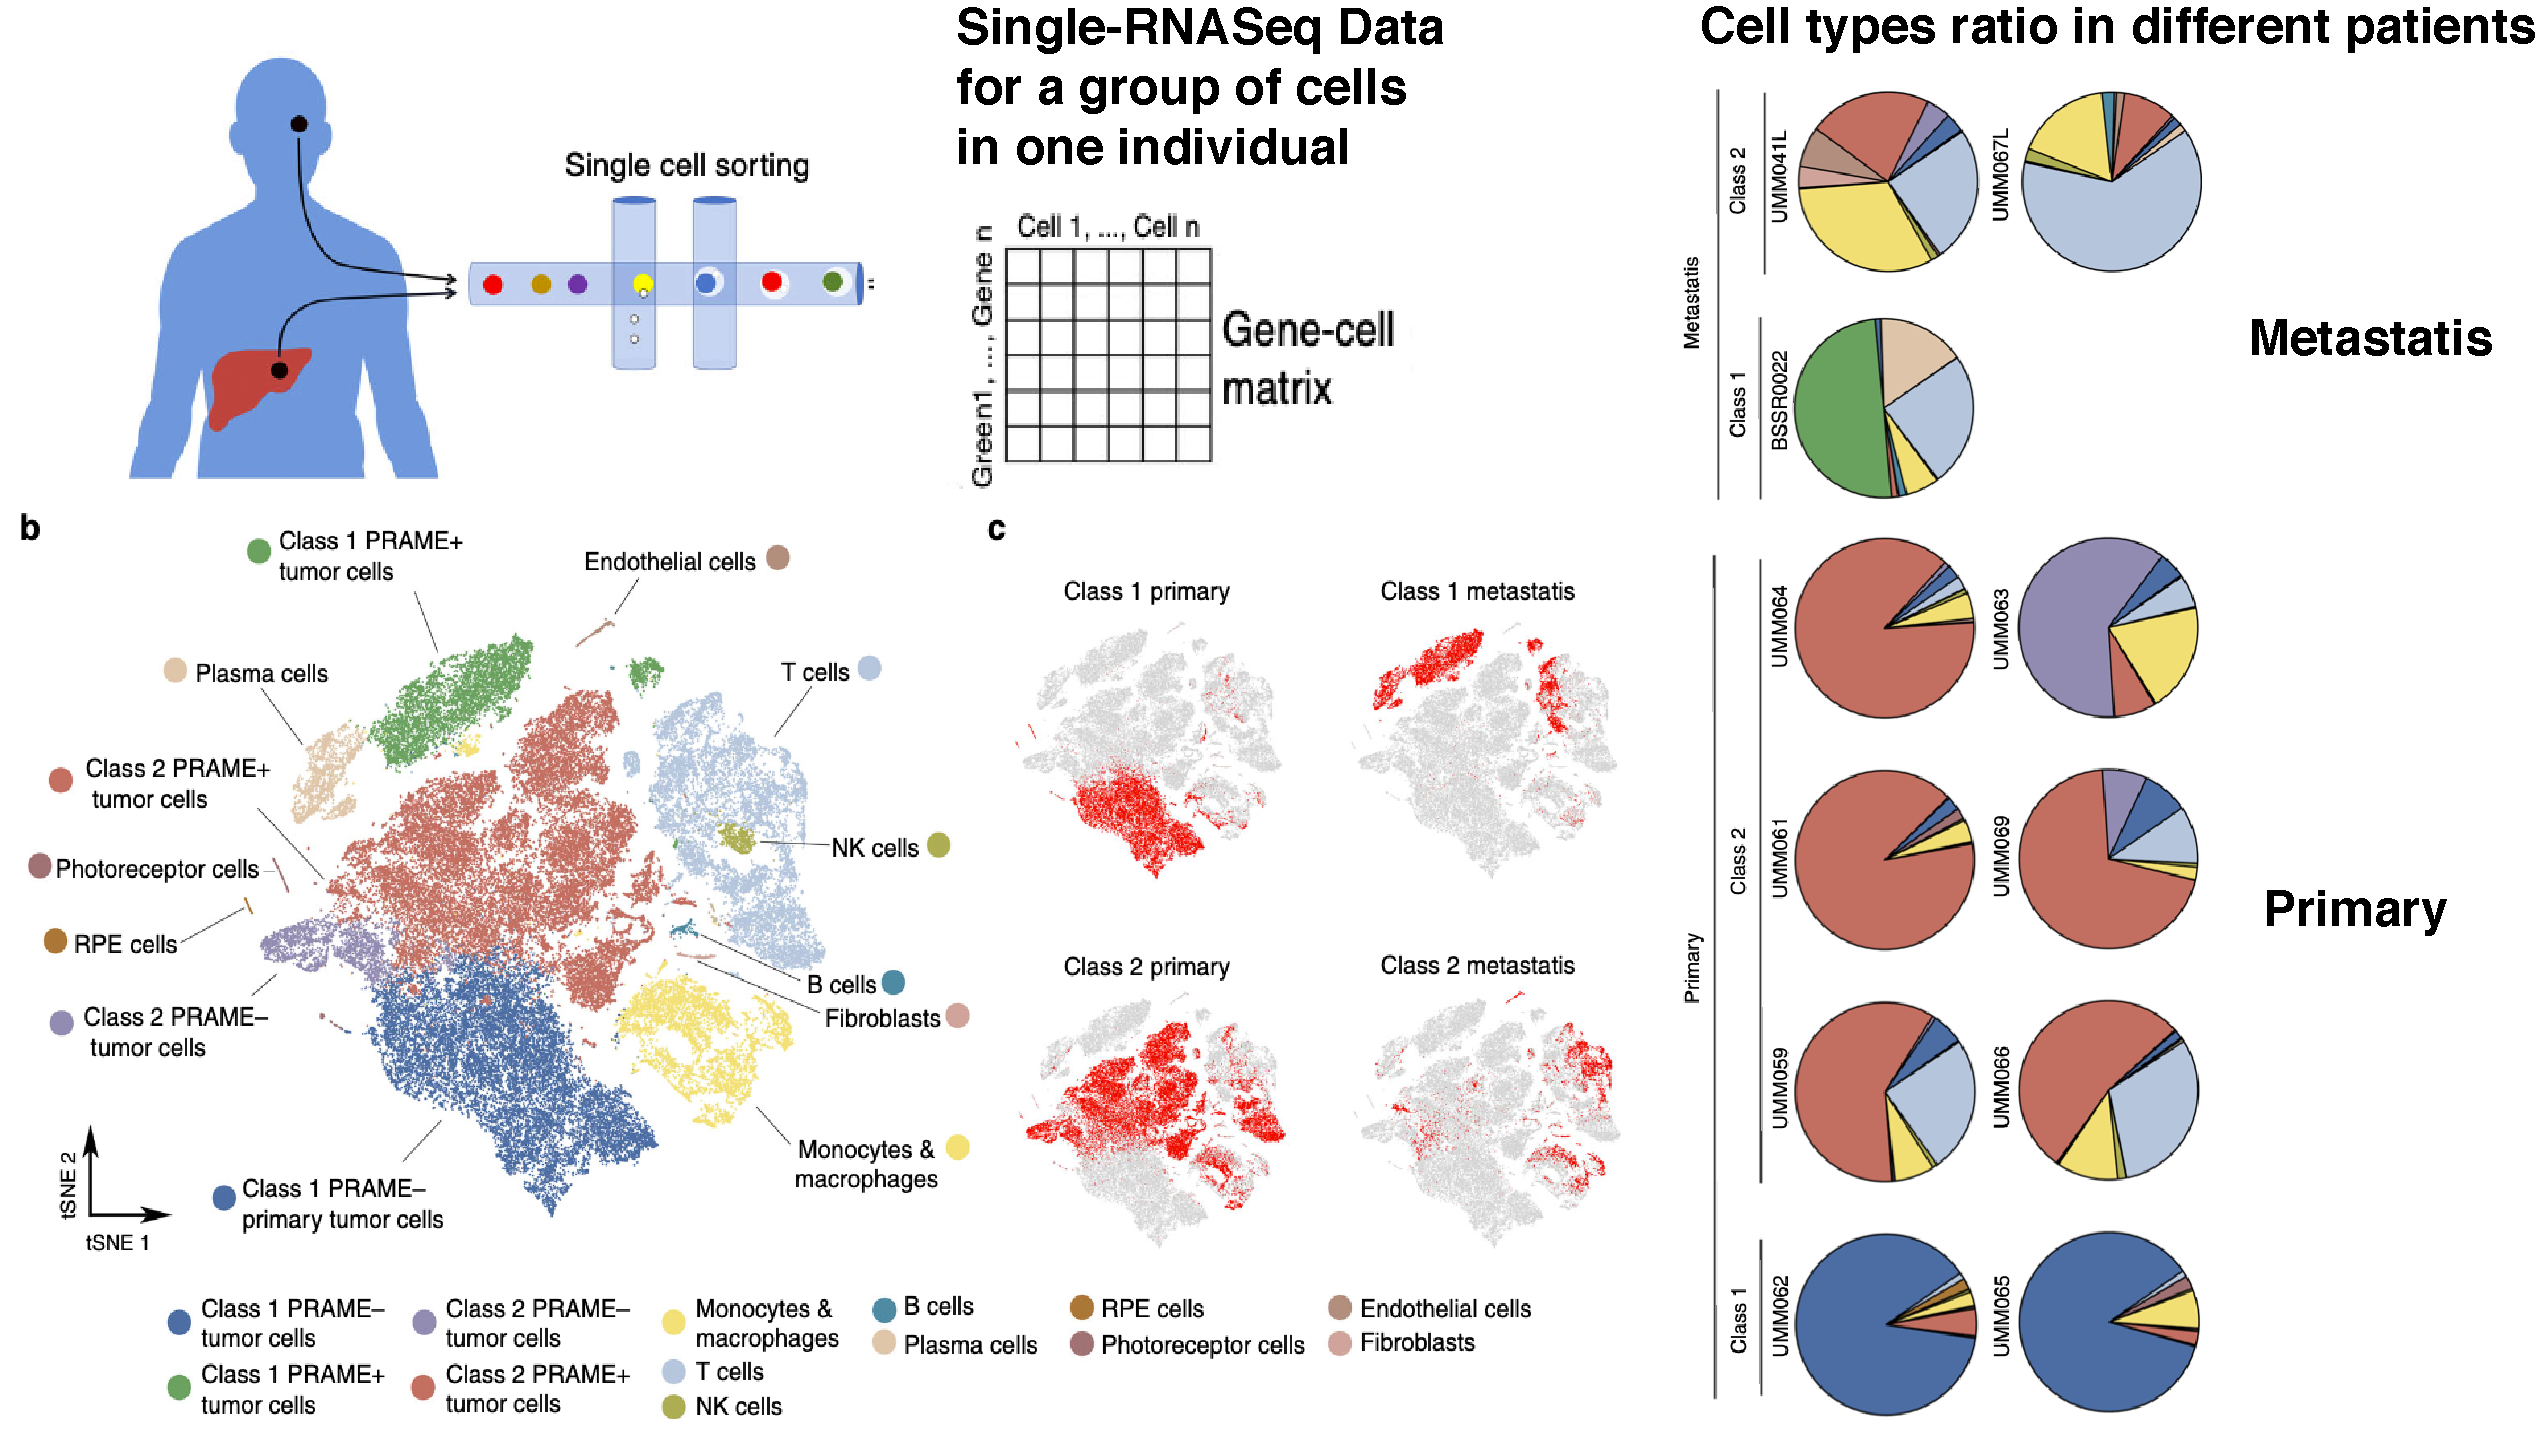
\includegraphics[width = \textwidth]{intro_overview}
    \caption{Multiple-sample scRNAseq Data \cite{durante2020single}.}
  \end{figure}
\end{frame}

\begin{frame}
  \begin{figure}
    \centering
    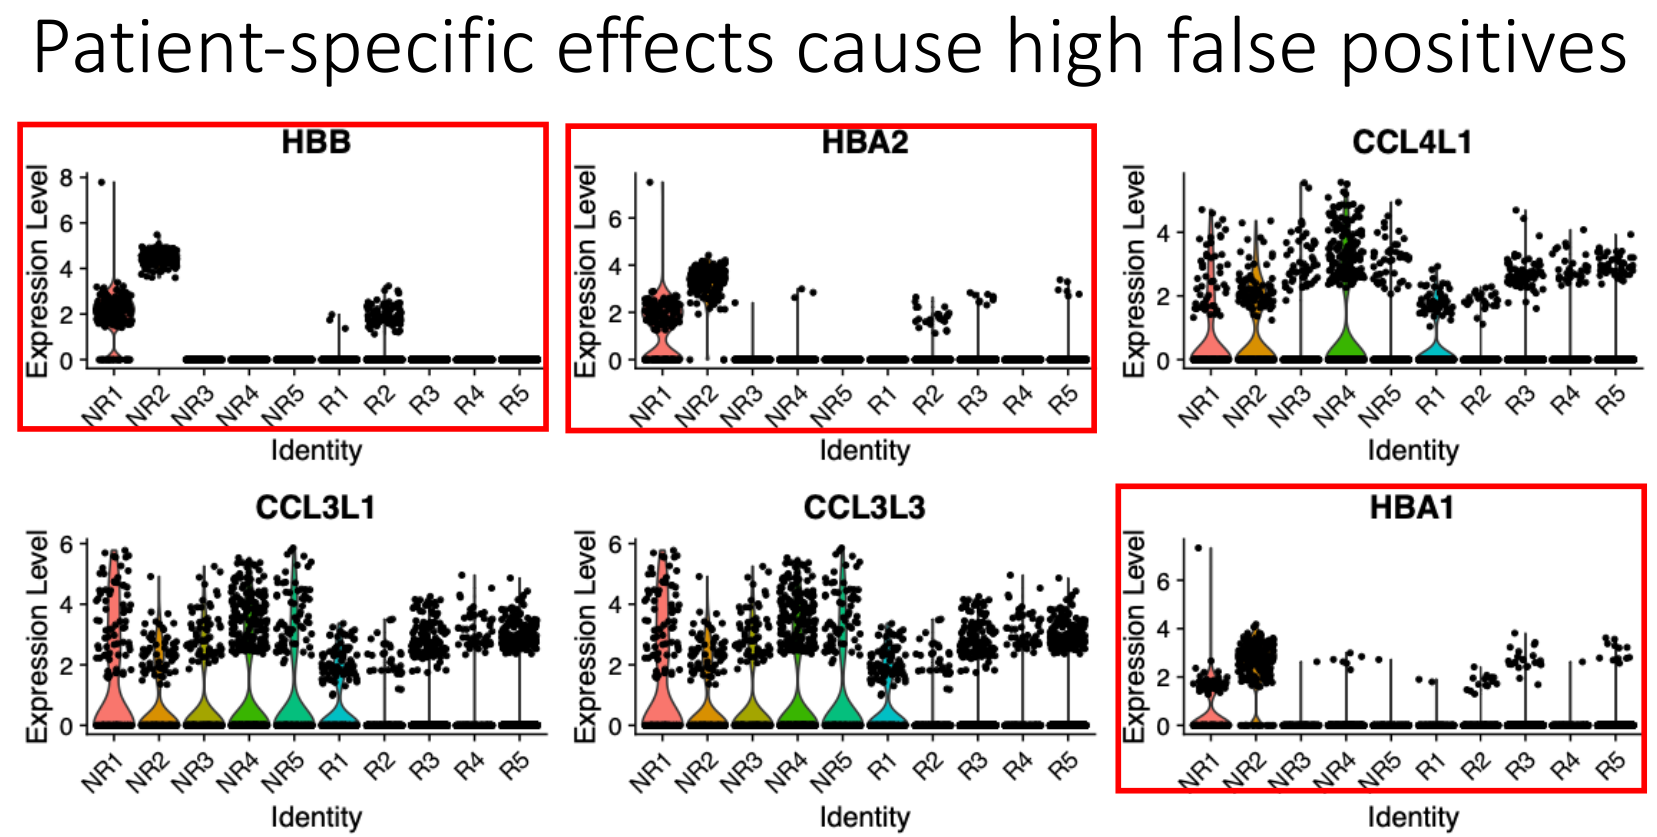
\includegraphics[width = 0.9\textwidth]{patient-specific.png}
    \caption{DE analysis on one cell sub-population inferred by Harmony
      \cite{korsunsky2019fast}}
  \end{figure}
\end{frame}

\begin{frame}
  \begin{figure}
    \centering
    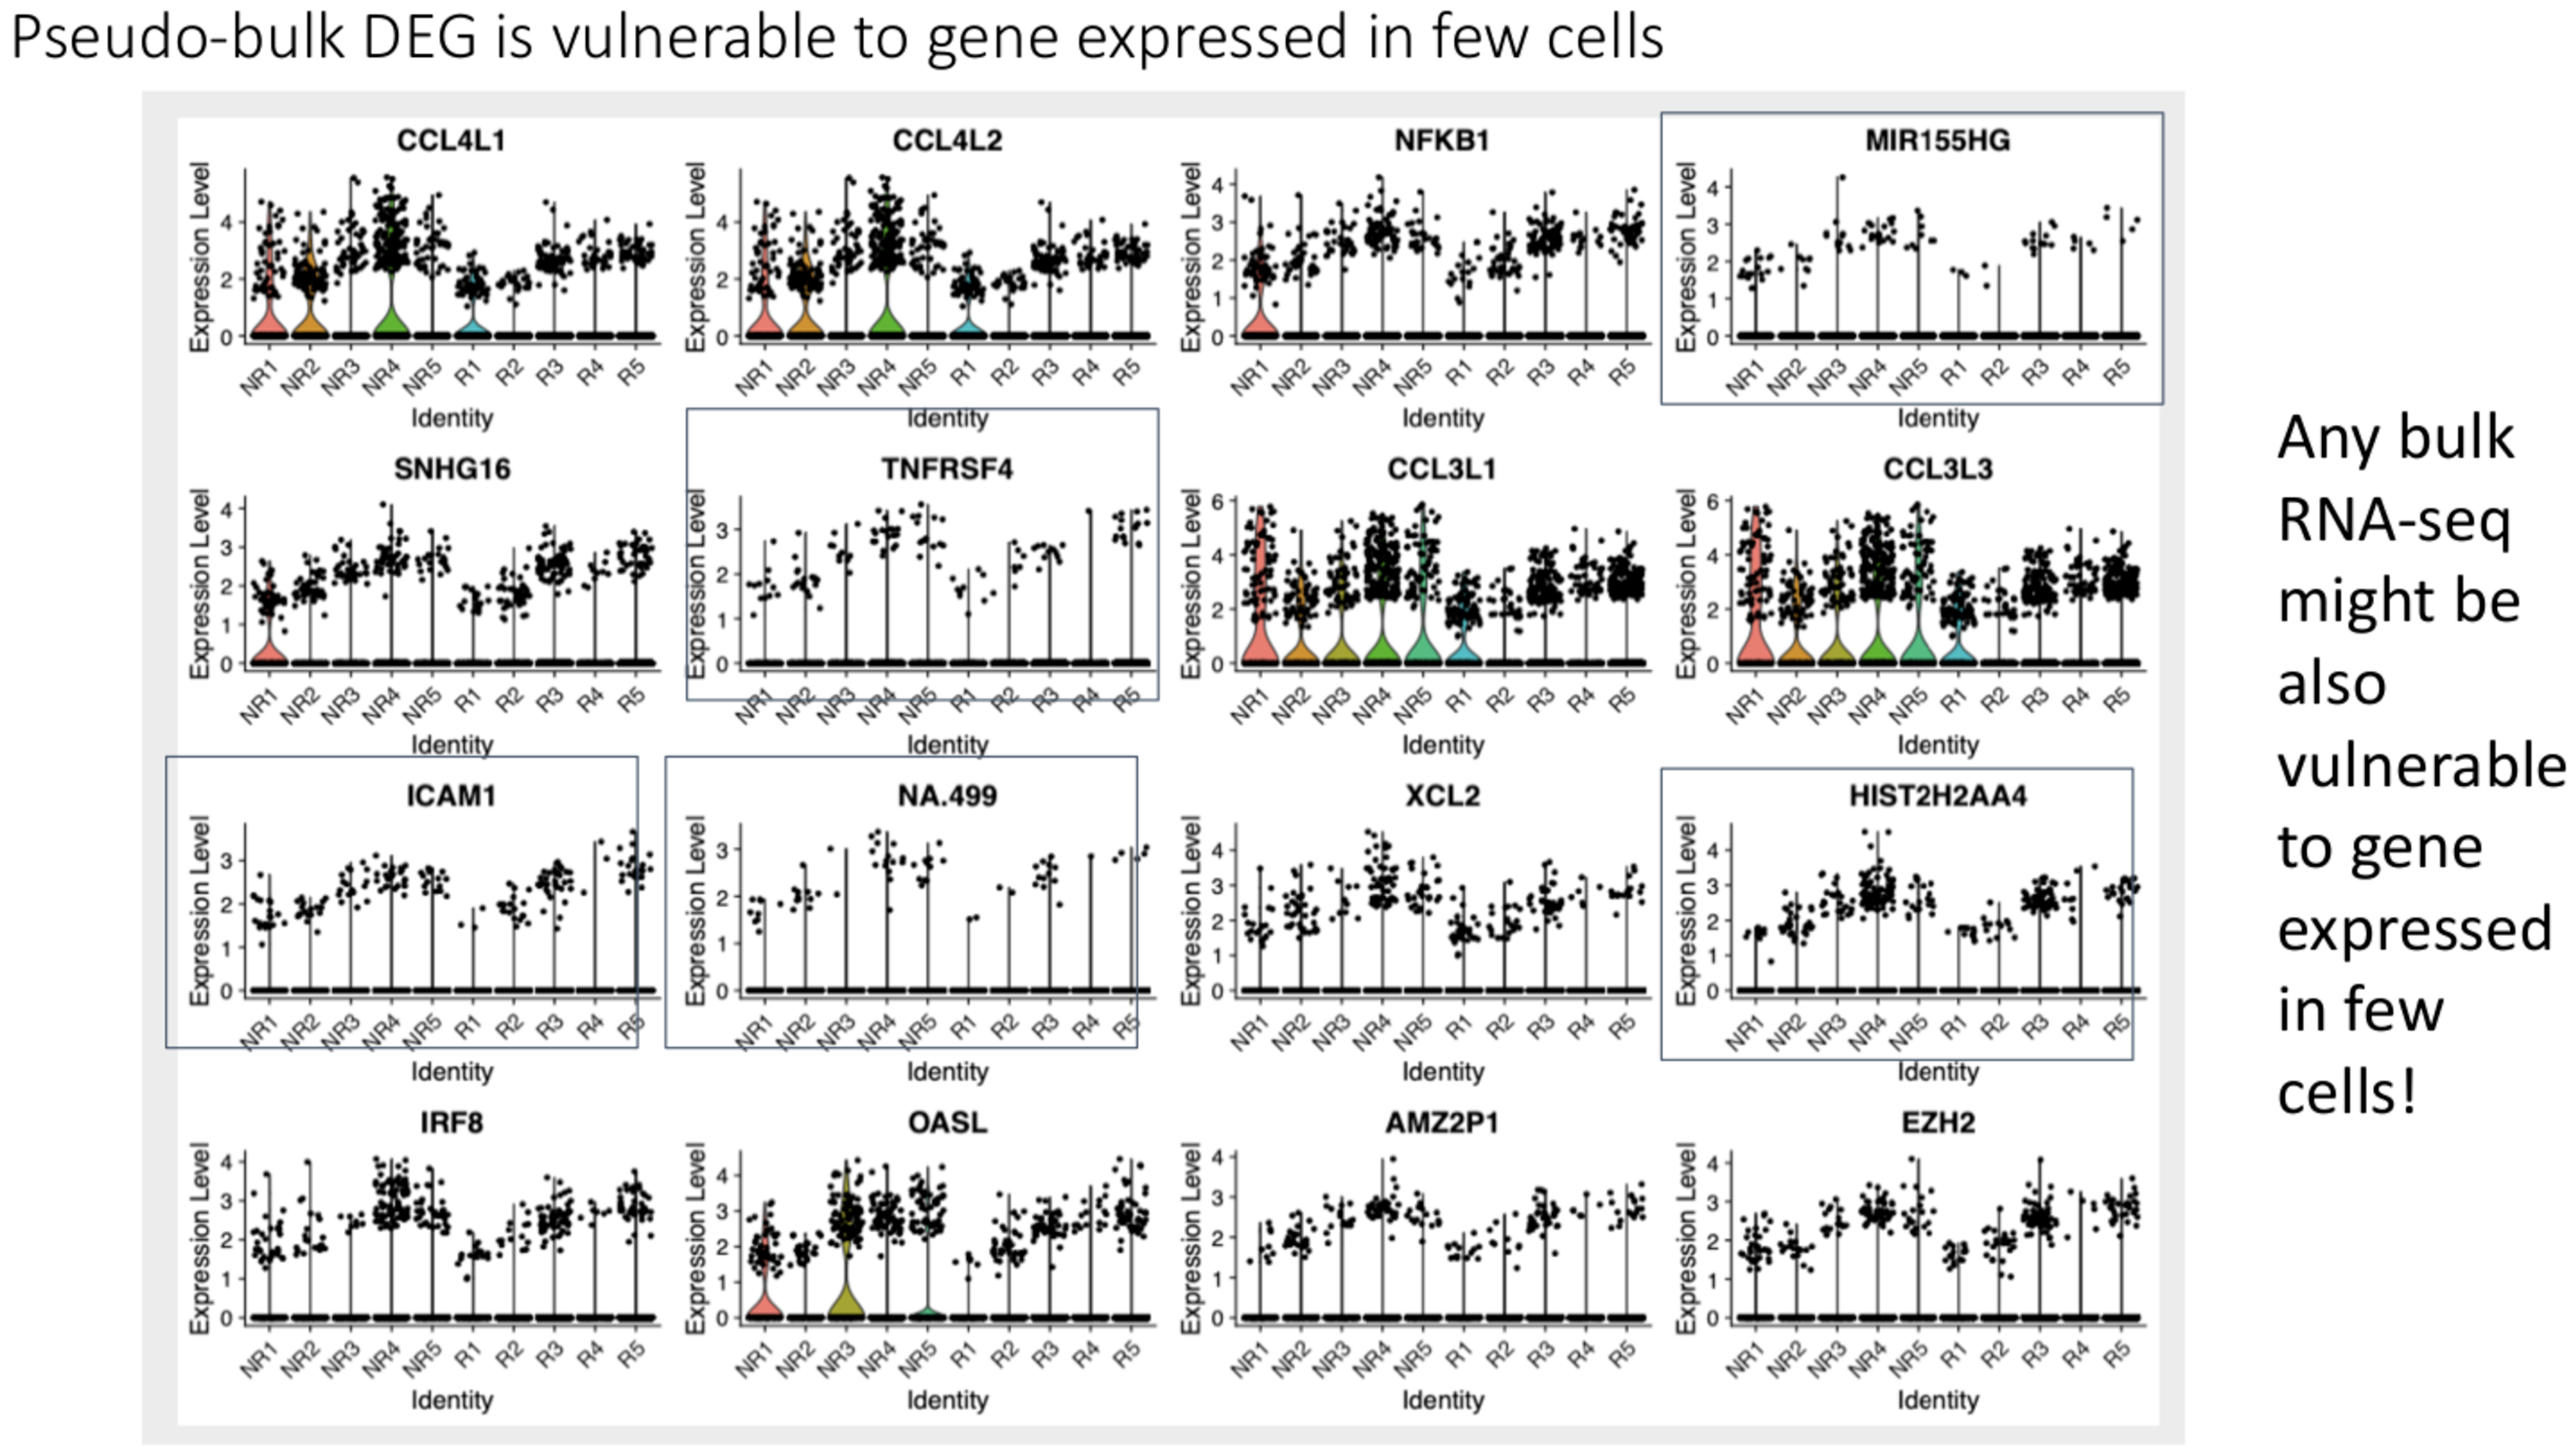
\includegraphics[width=\textwidth]{pseudobulkwhenmorezeros}
    \caption{Pseudo-bulk analysis \cite{schmid2020design} on PBMC dataset.}
  \end{figure}
\end{frame}

